\documentclass[tikz,border=4pt]{standalone}
\usepackage{amsmath,amssymb}

\usetikzlibrary{arrows.meta,positioning,automata,shapes,shapes.misc,calc,decorations.pathmorphing,decorations.markings,angles,quotes,patterns,mindmap,matrix,knots,hobby,trees}
\tikzset{->-/.style={decoration={markings, mark=at position 0.5 with {\arrow{Stealth}}}, postaction={decorate}}}
\begin{document}
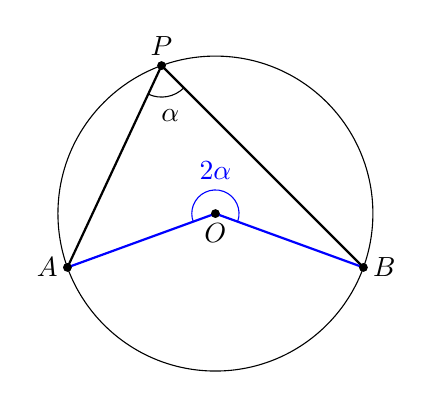
\begin{tikzpicture}[scale=2]
\draw (0,0) circle (1);
\coordinate (O) at (0,0); \coordinate (A) at (200:1); \coordinate (B) at (-20:1); \coordinate (P) at (110:1);
\draw[thick] (A) -- (P) -- (B); \draw[thick, blue] (A) -- (O) -- (B);
\foreach \p/\pos in {O/below, A/left, B/right, P/above} { \fill (\p) circle (0.8pt); \node[\pos] at (\p) {$\p$}; }
\pic[draw, angle radius=4mm, "$\alpha$", angle eccentricity=1.6] {angle=A--P--B};
\pic[draw, blue, angle radius=3mm, "$2\alpha$", angle eccentricity=1.8] {angle=B--O--A};
\end{tikzpicture}
\end{document}
